\documentclass[aspectratio=169]{beamer}
\usepackage{graphicx}
\usepackage[hungarian]{babel}
\usepackage{hulipsum}
\usepackage{xcolor}
\usetheme{Madrid}

 \AtBeginSection{\frame{%
 \tableofcontents[currentsection]}}

\title{Készfeladat05.01}
\author{Viktor Soltész}
\date{November 2024}

\begin{document}

\frame[plain]{\maketitle}

\section{1 feladat}
\subsection

\begin{frame}{Csoki}
    \frametitle{Süti}
    Szeretem a csokit
   
\end{frame}

\begin{frame}{Pizza}
    \frametitle{hús}
    Szeretem a pizzát.
\end{frame}

\begin{frame}{Leves}
    \frametitle{Gulyás}
    Szeretem a gulyást.
\end{frame}

\subsection{f}

\begin{frame}[fragile]{Verbatim teszt}
    \frametitle{teszt}
    \begin{verbatim}
        \begin{frame}{Leves}
    \frametitle{Gulyás}
    Szeretem a gulyást.
    \end{verbatim}
\end{frame}

\subsection{g}

\begin{frame}[allowframebreaks]{zagyva}
    \hulipsum[1-3]
\end{frame}

\section{2. feladat}
\subsection{a}

\begin{frame}{Kétoszlopos teszt dia}
    \begin{columns}
        \column{0.5\linewidth}
            \begin{itemize}
                \item Első 
                
                \pause Szünet
                \item Második valami
            \end{itemize}
            
        \column{0.5\linewidth}
            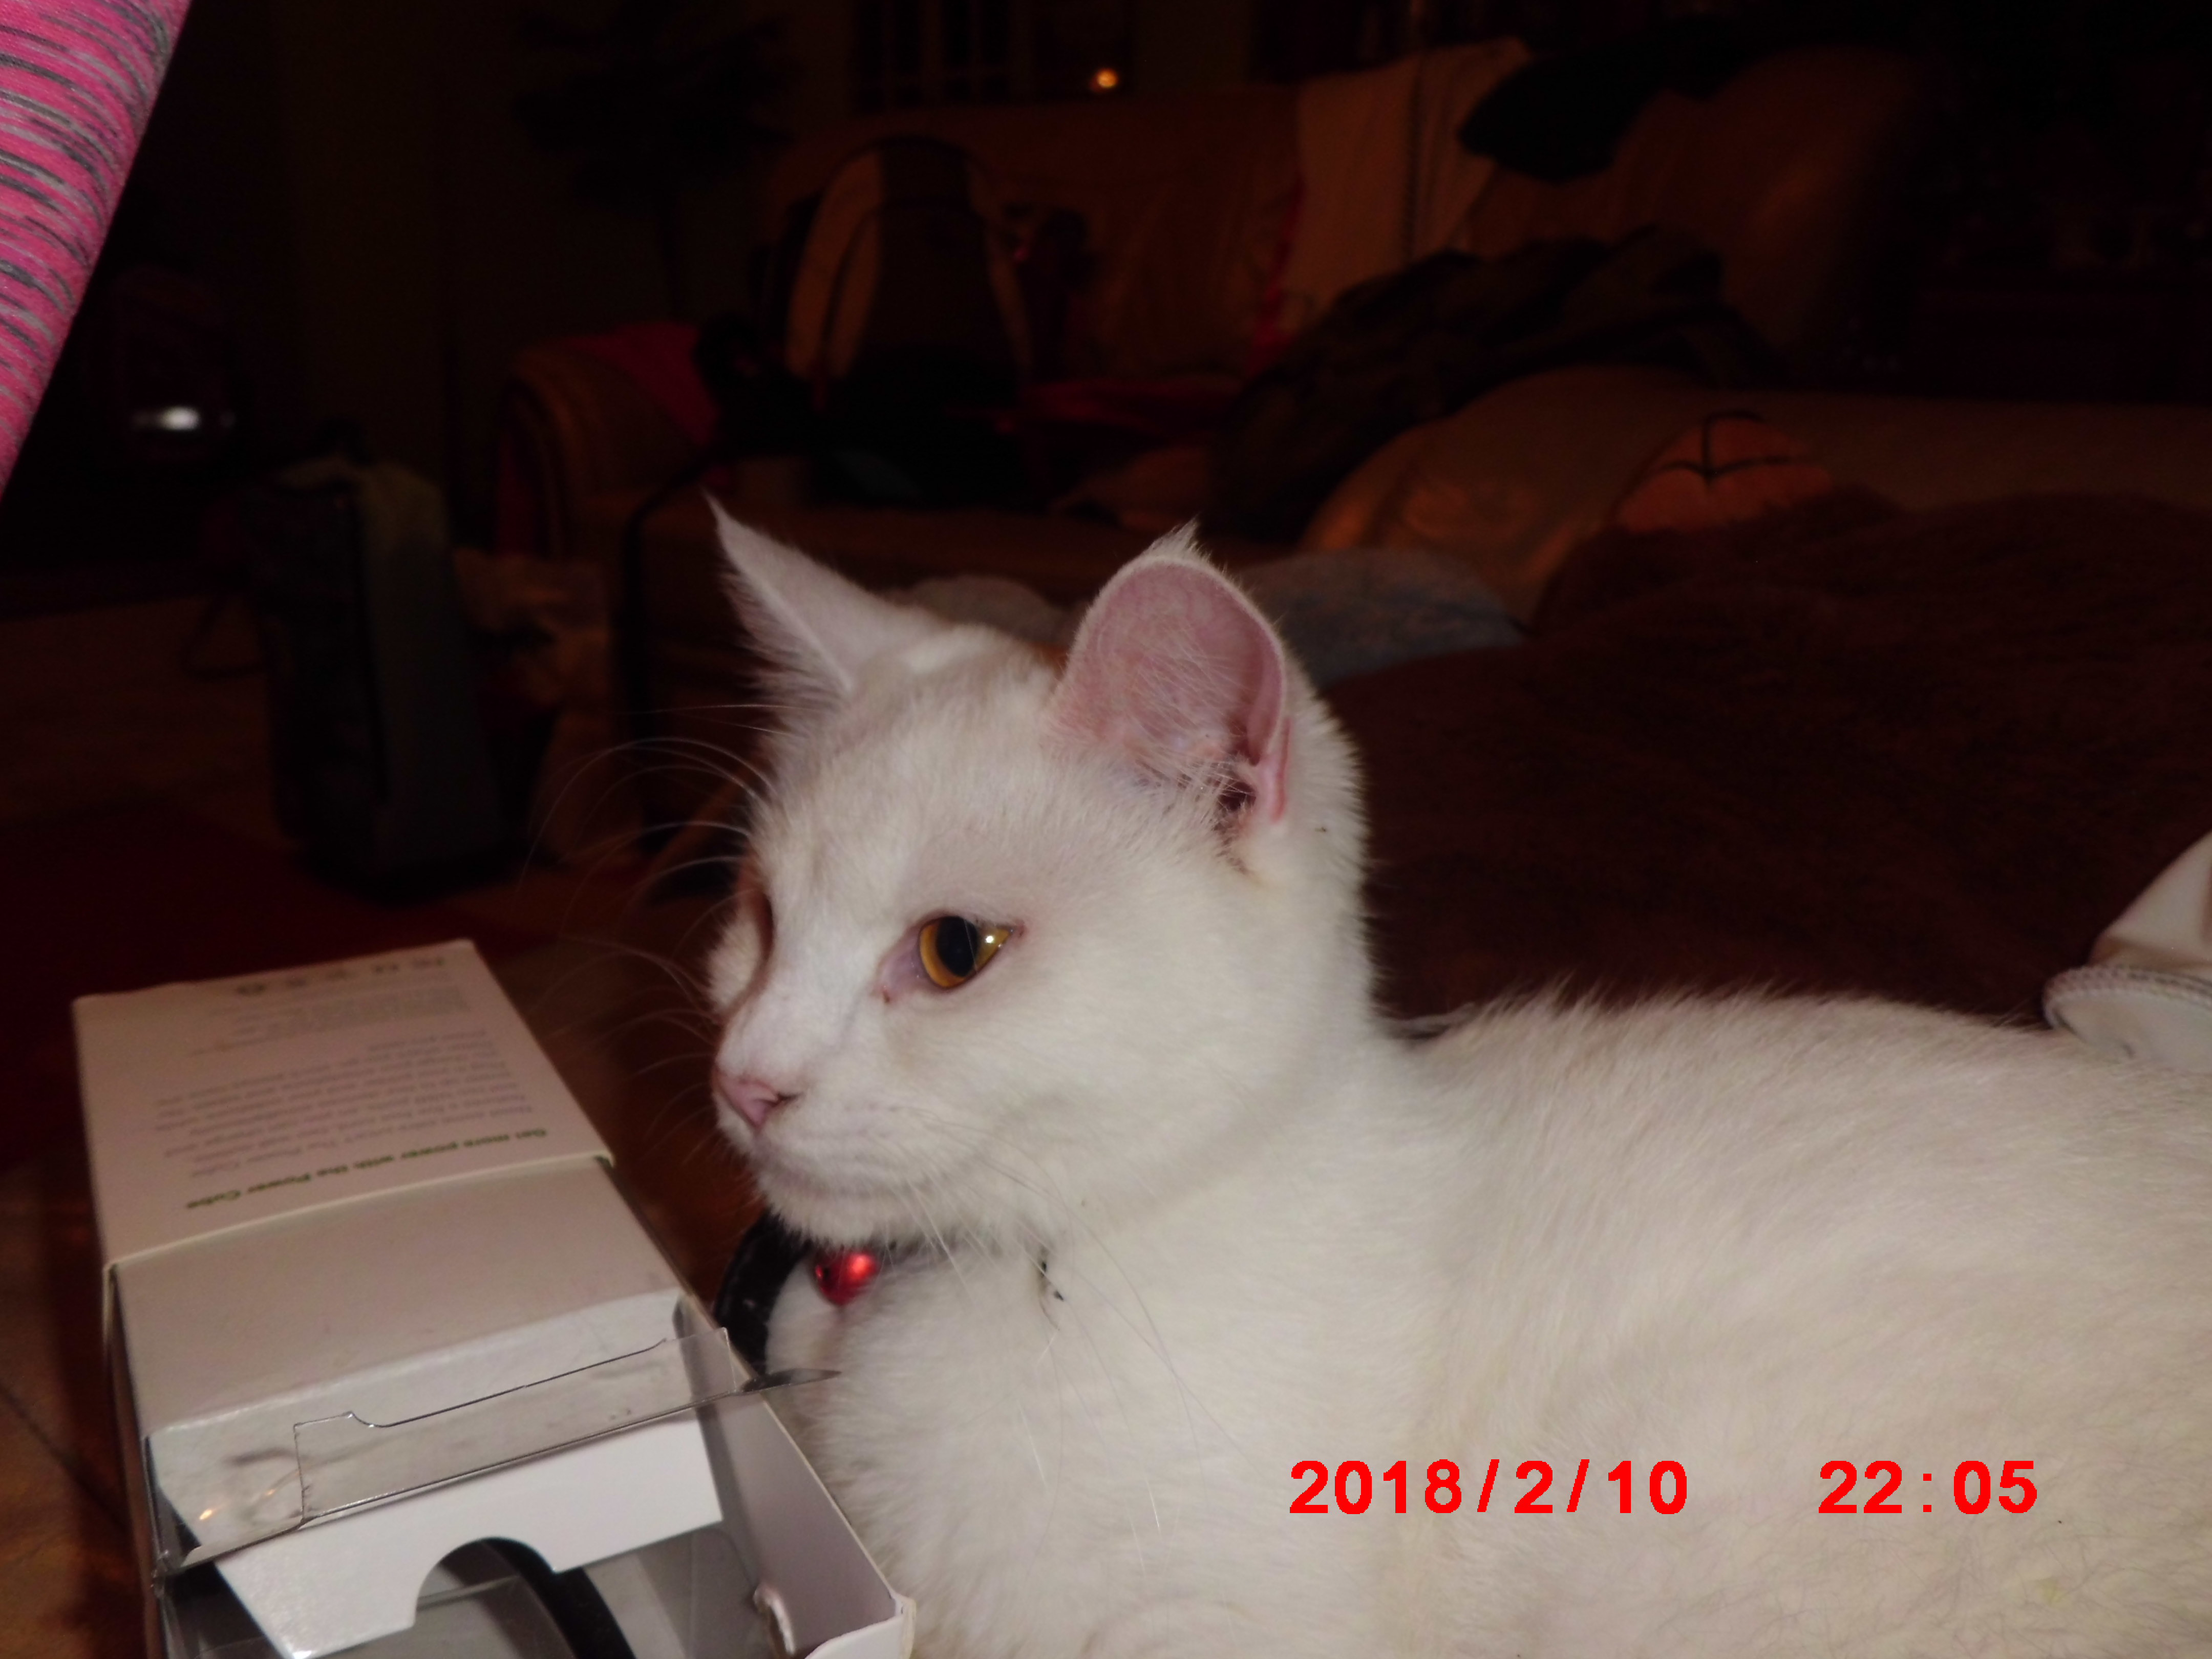
\includegraphics[width=\linewidth]{CIMG0595.JPG}
    \end{columns}
\end{frame}

\subsection{b}

\begin{frame}{Block teszt}
    \begin{block}
        Cím nélküli furcsa
    \end{block}
    \begin{exampleblock}{exampleblock címes}
        Ennek van címe
    \end{exampleblock}
    \begin{alertblock}{alertblock címes}
        Ennek is van címe
    \end{alertblock}
\end{frame}

\subsection{c}

\begin{frame}{Tétel és bizonyítás}
    \begin{theorem}[Szép tétel]
        Valmi tétel pl.
    \end{theorem}
    \begin{proof}<2->[szép biz]
        \hulipsum[1]
    \end{proof}
\end{frame}

\subsection{d}

\begin{frame}[fragile]{Semiverbatim teszt}
\transfade
    \begin{semiverbatim}
            \textcolor{red}{\\begin{frame}{Leves}}
            \textcolor{yellow}{\\frametitle{Gulyás}}
    
    Szeretem a gulyást.
    \end{semiverbatim}
\end{frame}

\begin{frame}{Képek váltakozása}
    \frametitle{Cuki cica}
    \transdissolve<1,2>
    \only<1>{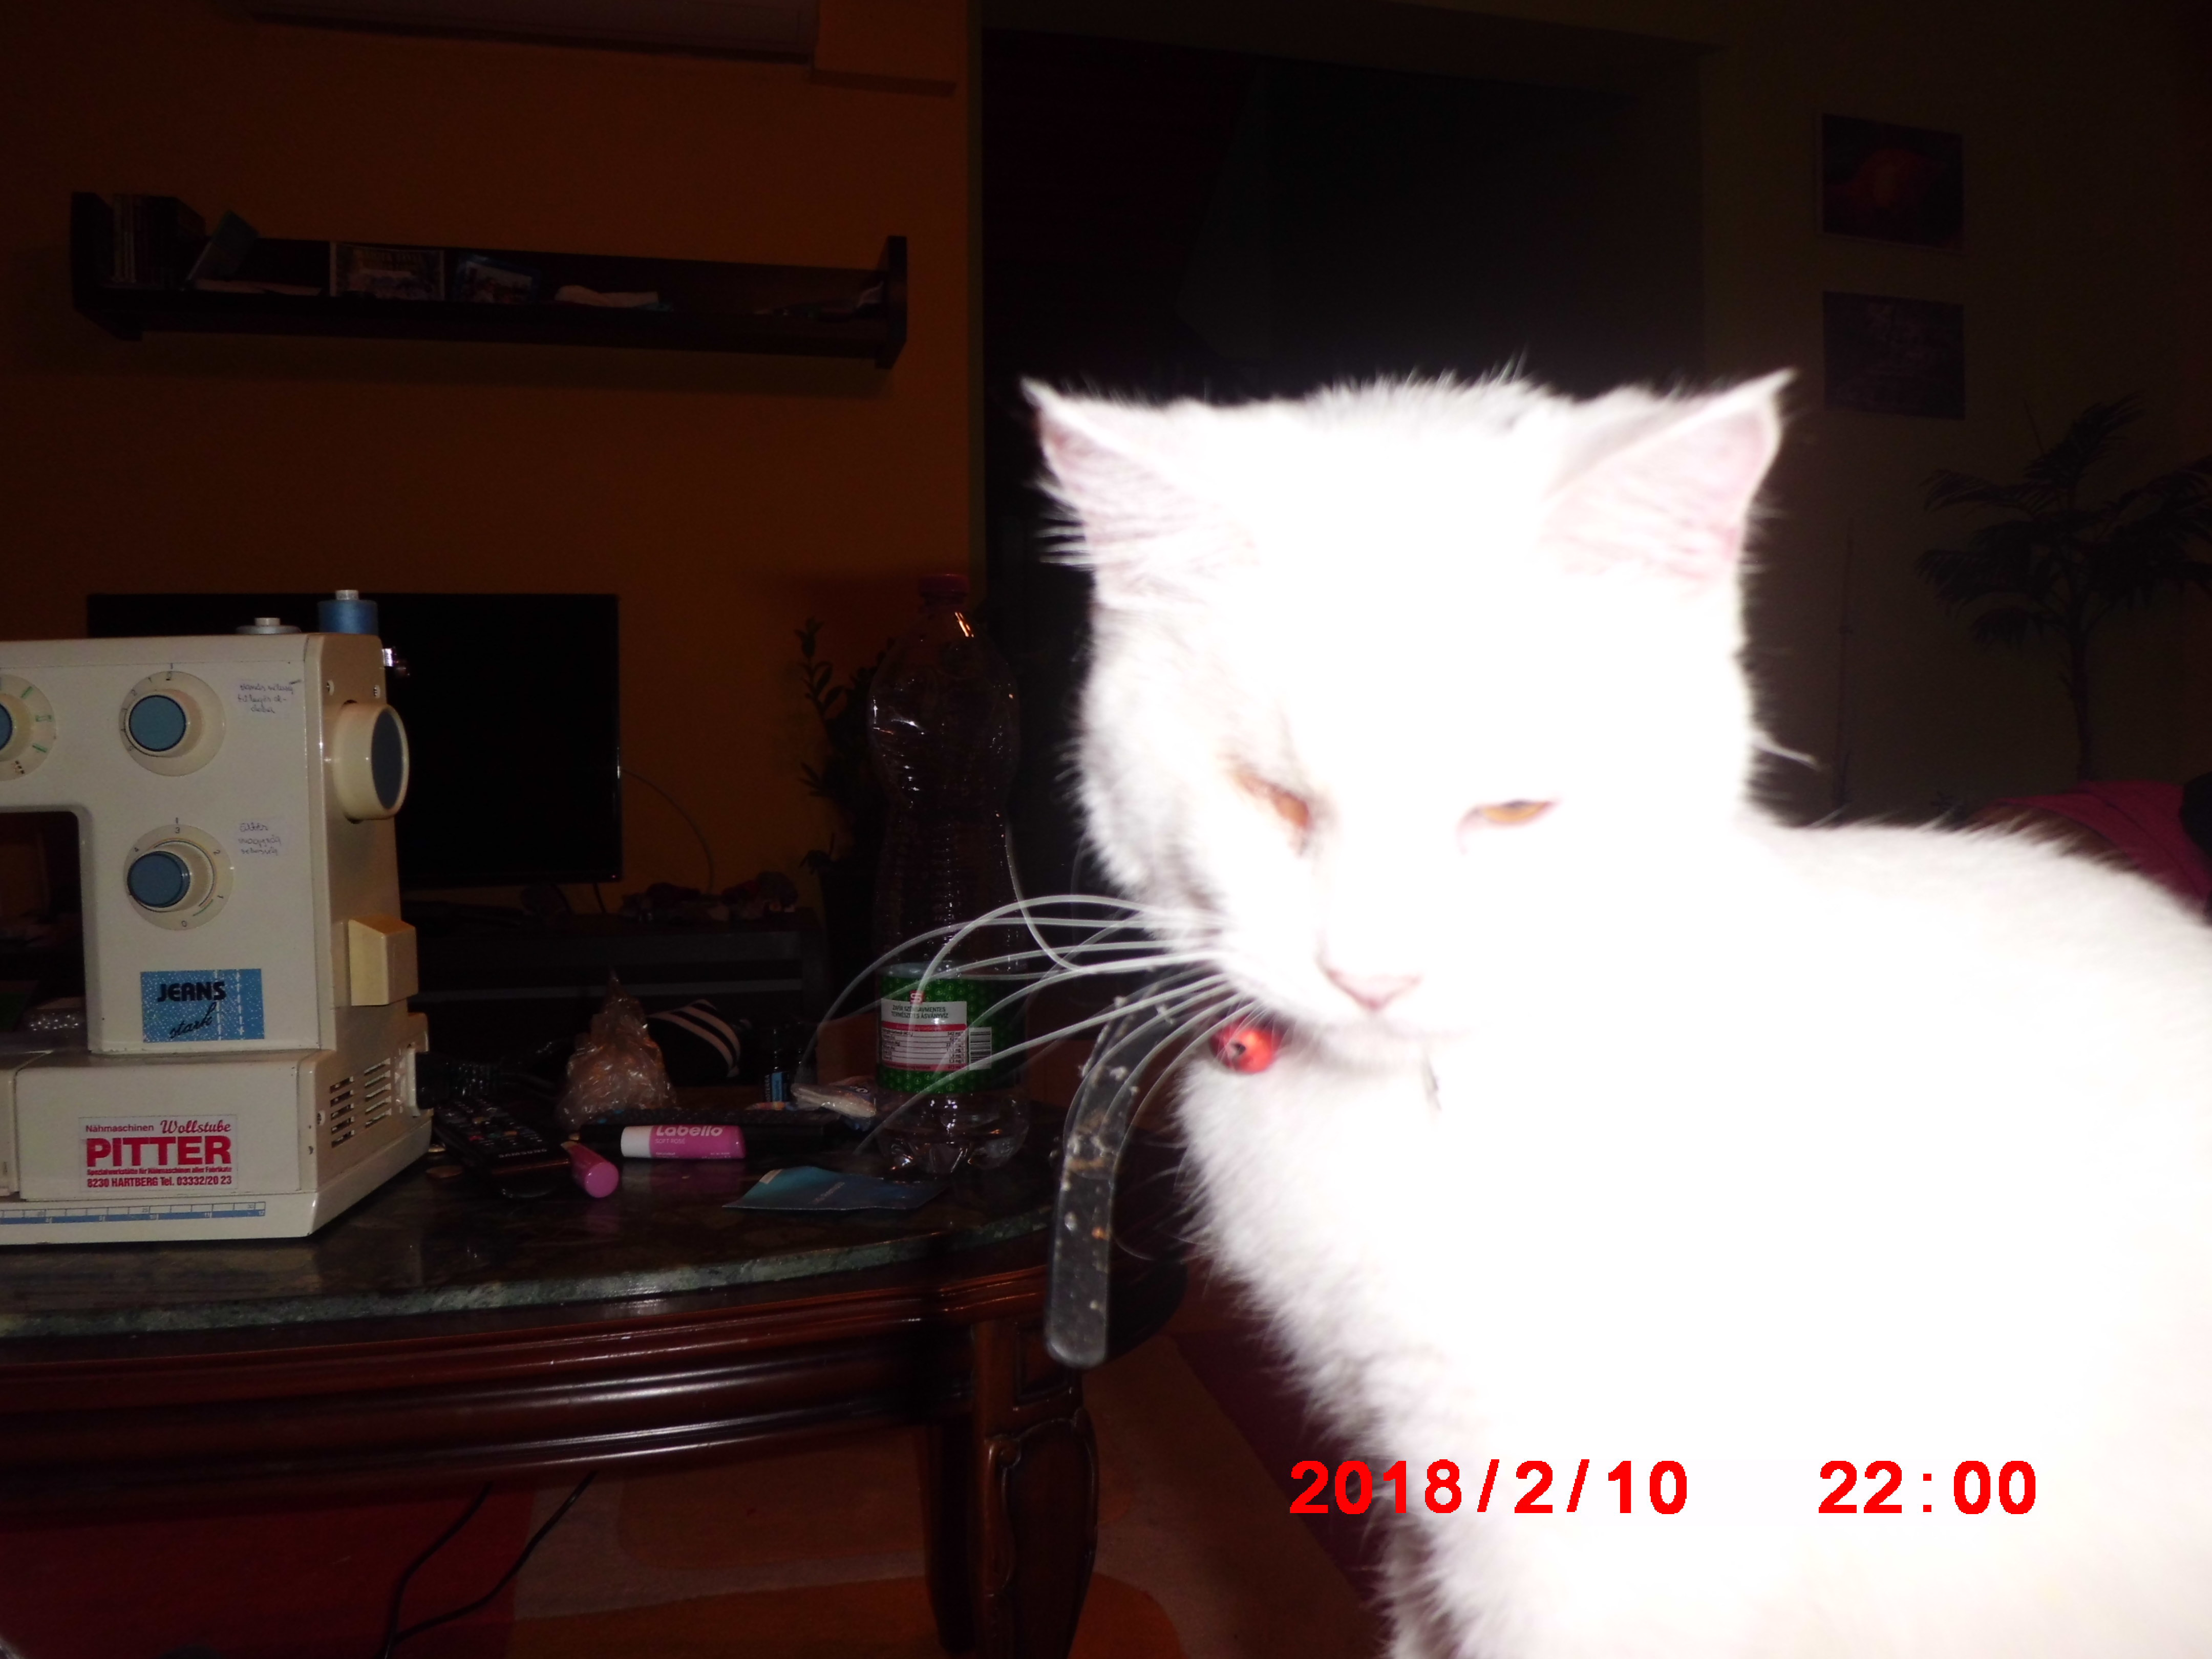
\includegraphics[width=0.8\textwidth]{CIMG0594.JPG}}
    \only<2>{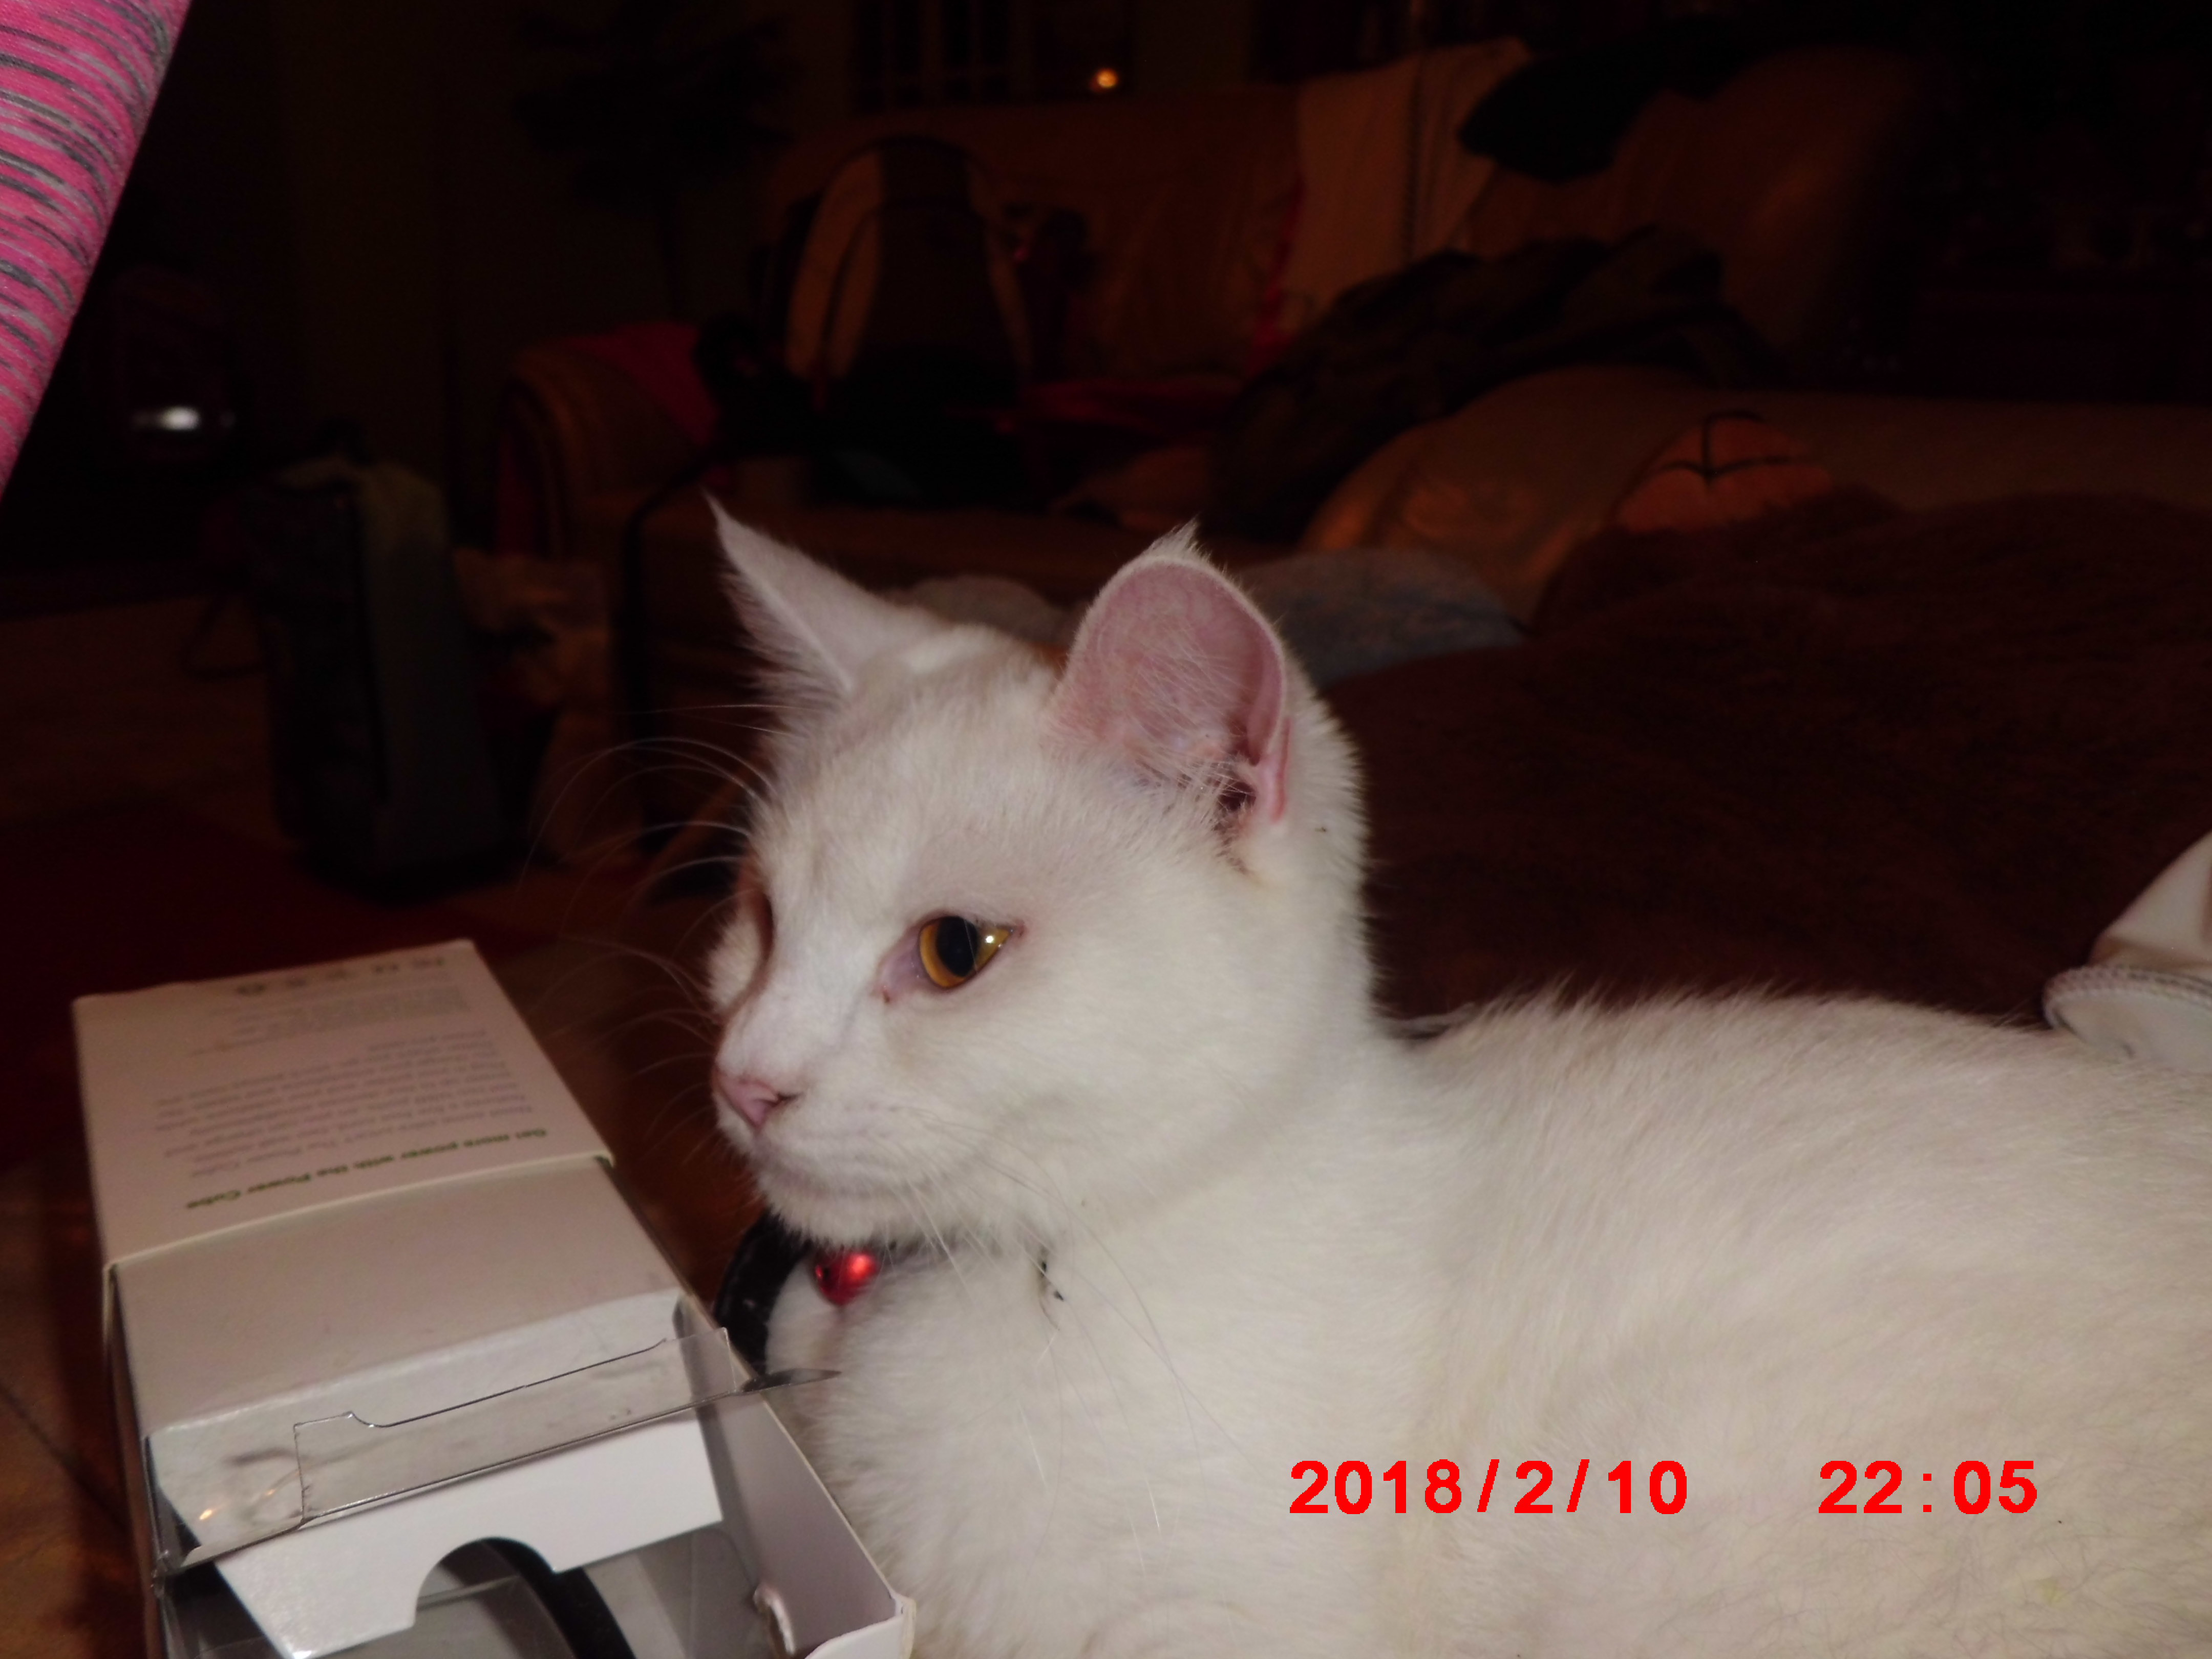
\includegraphics[width=0.8\textwidth]{CIMG0595.JPG}}

\end{frame}

\end{document}
